\documentclass[10pt,letterpaper]{article}
\usepackage[margin=0.7in]{geometry}
\usepackage{graphicx,booktabs,tabularx,array,longtable}
\usepackage[T1]{fontenc}
\usepackage[hidelinks]{hyperref}
\usepackage{url}
\Urlmuskip=0mu plus 1mu\relax
\setlength{\parindent}{0pt}
\setlength{\parskip}{6pt}
\newcommand{\file}[1]{\nolinkurl{#1}}
\begin{document}
{\Large\bfseries Alluvial-ridge reproduction: scientific progress assessment}\par
12 October 2026\quad Independent Nicholas et al. (2018) investigation

\textbf{Decision.} A functioning independent channel--floodplain simulation and traceable first-flood validation outputs exist. Quantitative reproduction is not established: none of 13 manuscript panels has demonstrated agreement, and only one has partial requested data. The principal obstacle is numerical accuracy. Doubling floodplain spacing changes first-flood water storage by $-63\%$ and ridge height by $+155\%$. Stop open-ended development spending. At most, approve one bounded, scientist-led review of existing results before considering further calculations. Past expenditure is not evidence of future scientific return.

\textbf{Physical capabilities.} The model couples one-dimensional channel flow to two-dimensional floodplain shallow-water flow, transporting three suspended sediment classes through common water and sediment fluxes. It includes settling, shear-dependent cohesive deposition, diffusion, prescribed channel-bed aggradation, migration, cutoffs, and bank-sediment recycling. Existing outputs demonstrate flooding and deposition; saved checks support conservative transport and restart continuity. These capabilities support transport and sensitivity studies.

The domain is $72\times48$ km, with a 500 m channel, initial depth 8 m, and slope $10^{-4}$. Each prescribed 20-day flood spans 2,500--15,000 m$^3$ s$^{-1}$. Assumptions include a sinusoidal hydrograph, characteristic inlet and normal-depth outlet, initially dry floodplain, no hydraulic spinup, zero vertical floodplain entrainment, and zero net channel-bed exchange with suspension. Sediment concentration units, settling parameters, deposition threshold, and migration rules require interpretation beyond the written specification. These choices are documented, but their physical adequacy is unestablished.

\textbf{Direct numerical evidence.} Table 1 uses corrected, archived run-11 summaries; channel spacing remains 250 m. Ridge height is a longitudinal diagnostic, not a manuscript cross-section. Here $\alpha$ is mean floodplain depth divided by inundated bank fraction; $\beta$ is ridge height divided by channel depth.

\begin{center}\small
\begin{tabular}{lrrr}\toprule
Quantity & 250 m floodplain & 500 m floodplain & Change\\\midrule
Day-12 $\alpha$ (m)&0.88449&0.77058&$-12.9\%$\\
Day-20 ridge height (m)&0.01319&0.03357&$+154.6\%$\\
Day-20 $\beta$&0.001644&0.004178&$+154.2\%$\\
Water storage ($10^6$ m$^3$)&555.865&207.258&$-62.7\%$\\
Recorded water residual (m$^3$)&$-1.96\times10^{-5}$&$-9.33\times10^{-5}$&---\\
Recorded sediment residual (kg)&$-0.754$&$-0.337$&---\\\bottomrule
\end{tabular}\par
Table 1. First-flood sensitivity, before geometry remapping. Small residuals establish neither spatial accuracy nor convergence.
\end{center}

\textbf{Repository assessed.} Baseline commit \texttt{e6bd002bdc83c0cd37ebede19ad29a9b6e487851}, branch \texttt{master}; no tracked modifications at inspection. Two untracked validation directories contained older runs and renderer checks. Their useful evidence is preserved separately with provenance (Appendix). The physical model is unchanged.

\newpage
\begin{center}
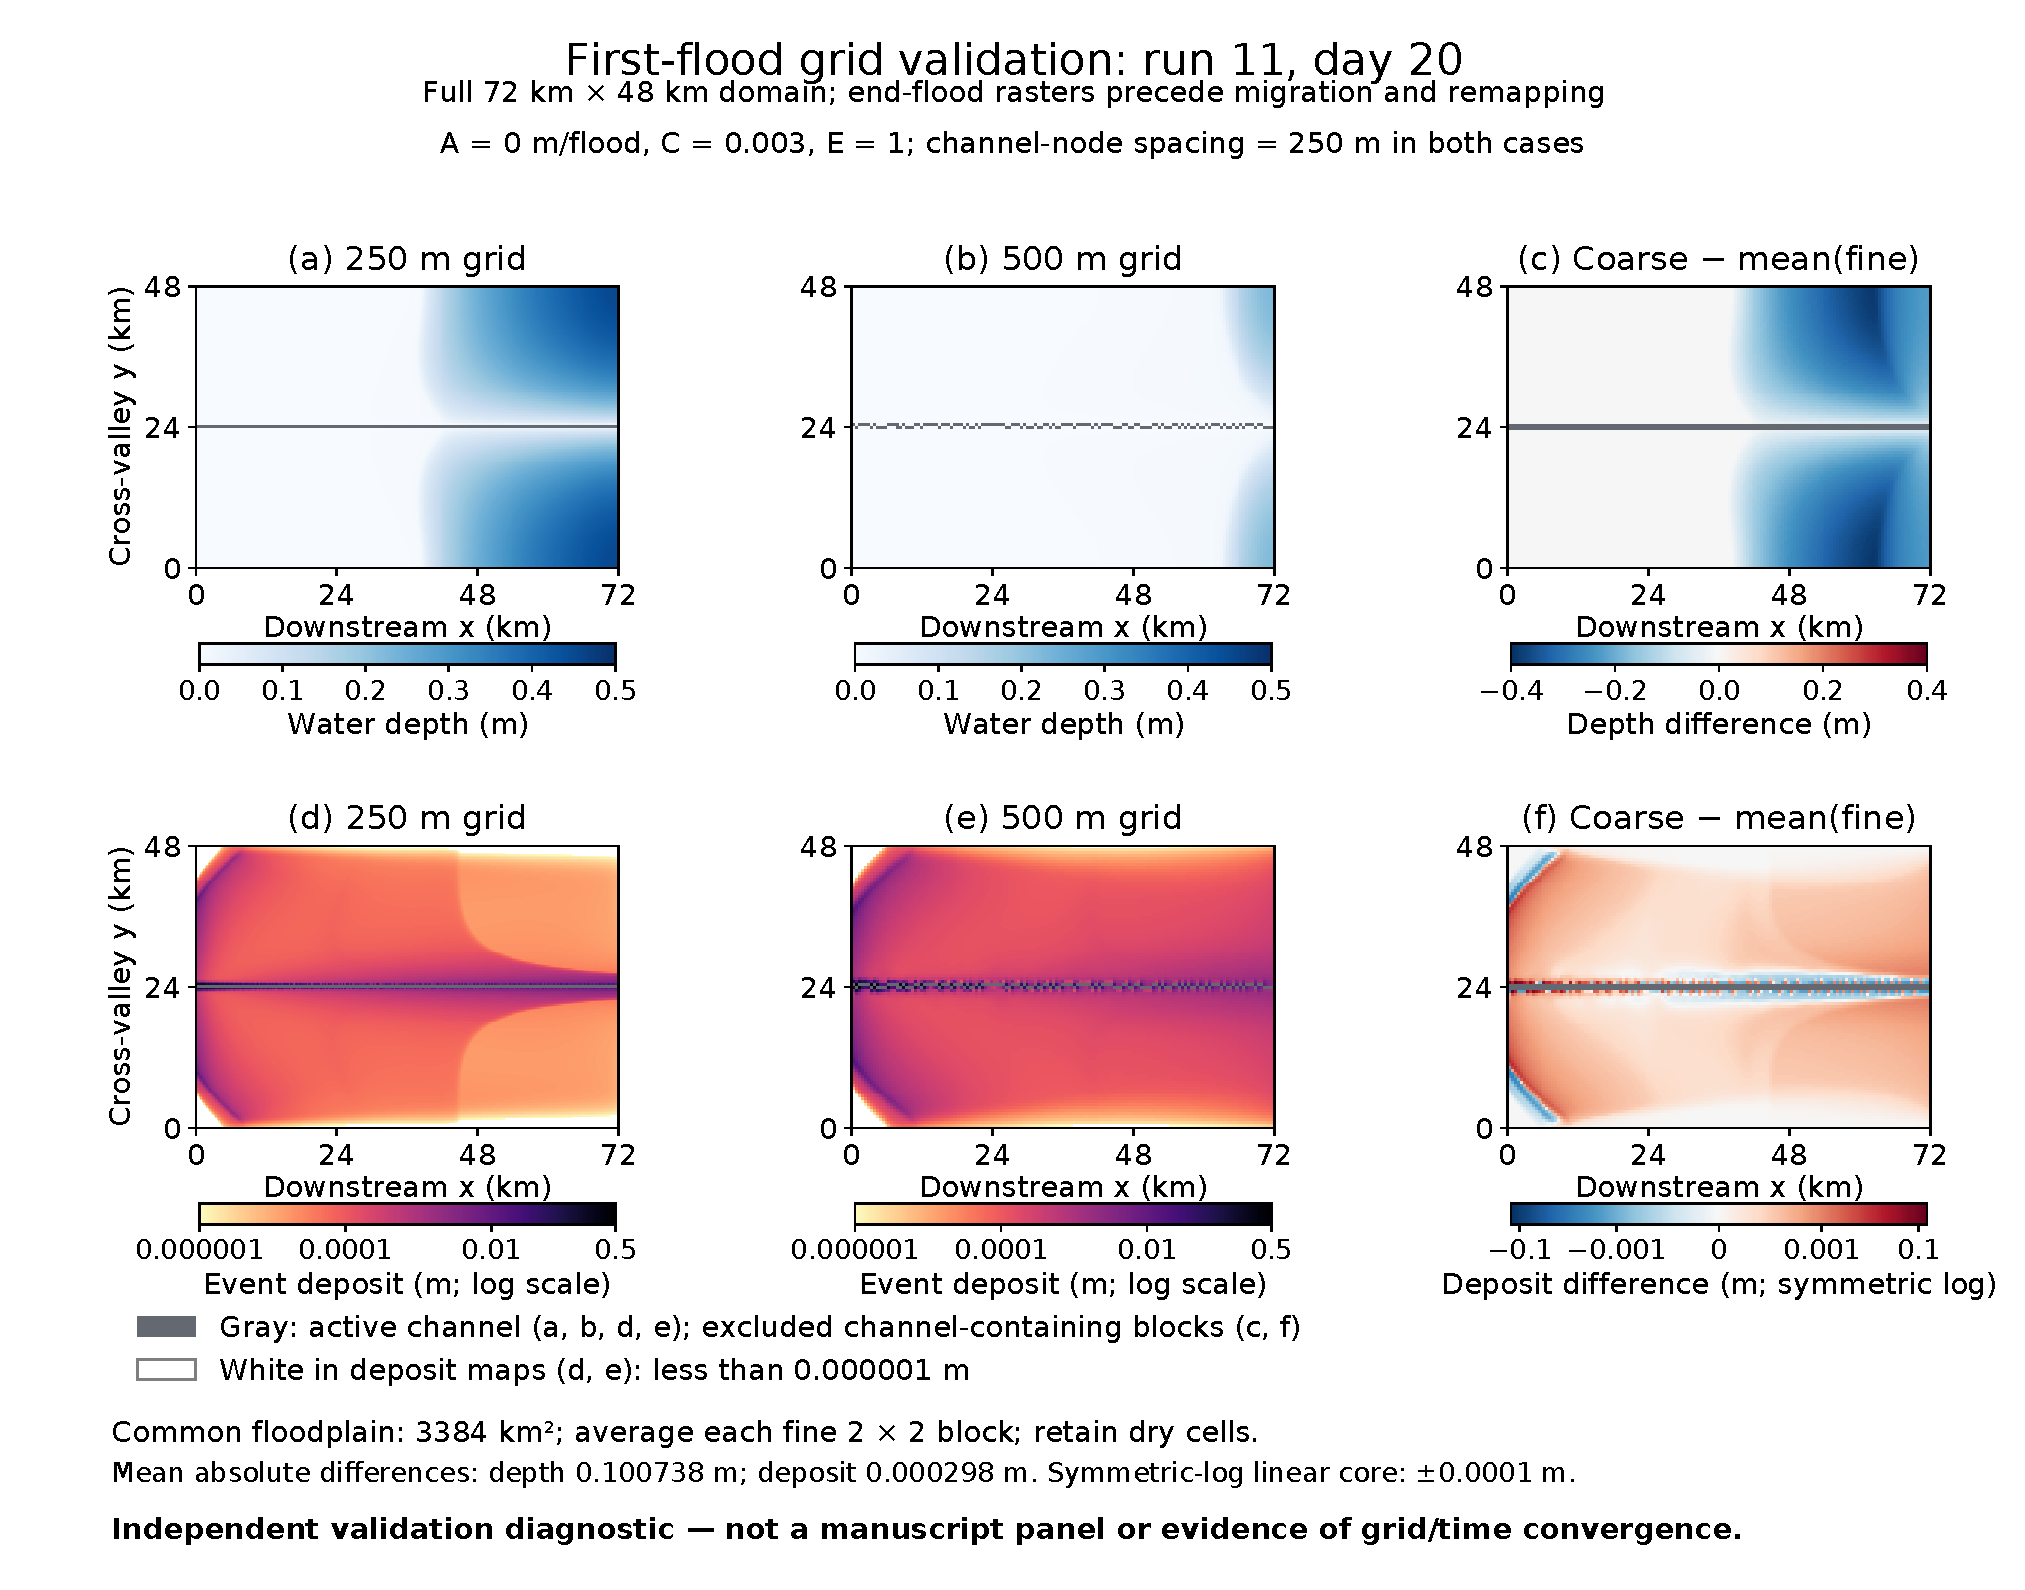
\includegraphics[width=\linewidth,height=5.1in,keepaspectratio]{figures/first_flood_validation.pdf}
\end{center}
\textbf{Figure 1.} Existing independently generated first-flood fields: 250 and 500 m water depth and deposition, and coarse-minus-averaged-fine differences. Axes are kilometres; color scales are metres. Deposit thickness uses logarithmic scales. Gray excludes channel-containing comparison blocks. The common floodplain area is 3,384 km$^2$. Mean absolute differences are 0.10074 m in water depth and 0.000298 m in deposit thickness. This is a validation figure, not a reproduced manuscript panel. Source: \file{figures/first_flood_validation.pdf} and its manifest.

\textbf{Credibility and its limits.} Thirty input, archive-member, and figure hash bindings were checked; archived summary values and early $\alpha$ statistics were recomputed. These checks connect the figures to saved independent data. Physical flux budgets were not independently reconstructed during this assessment.

Saved validation records cover lake at rest, normal flow, plume transport, settling, recycling, remapping, and restart equivalence. The inspected restart log records identical output files. In a documented 1,000 s normal-flow test, halving channel spacing reduced relative depth error from 0.001790 to 0.000843. This is a component result, not coupled-model convergence. Recorded first-flood refinement from 250 to 125 m changes storage by $+44.7\%$ and ridge height by $+109.7\%$; these finer-grid values were inspected in the saved assessment, not independently replayed here. Halving the CFL time-step limit changes saved storage by $-5.95\%$ and deposited mass by $-7.69\%$; these records were inspected, not replayed. No demonstrated convergence order or long-term error bound supports manuscript-scale conclusions.

\newpage
\begin{center}
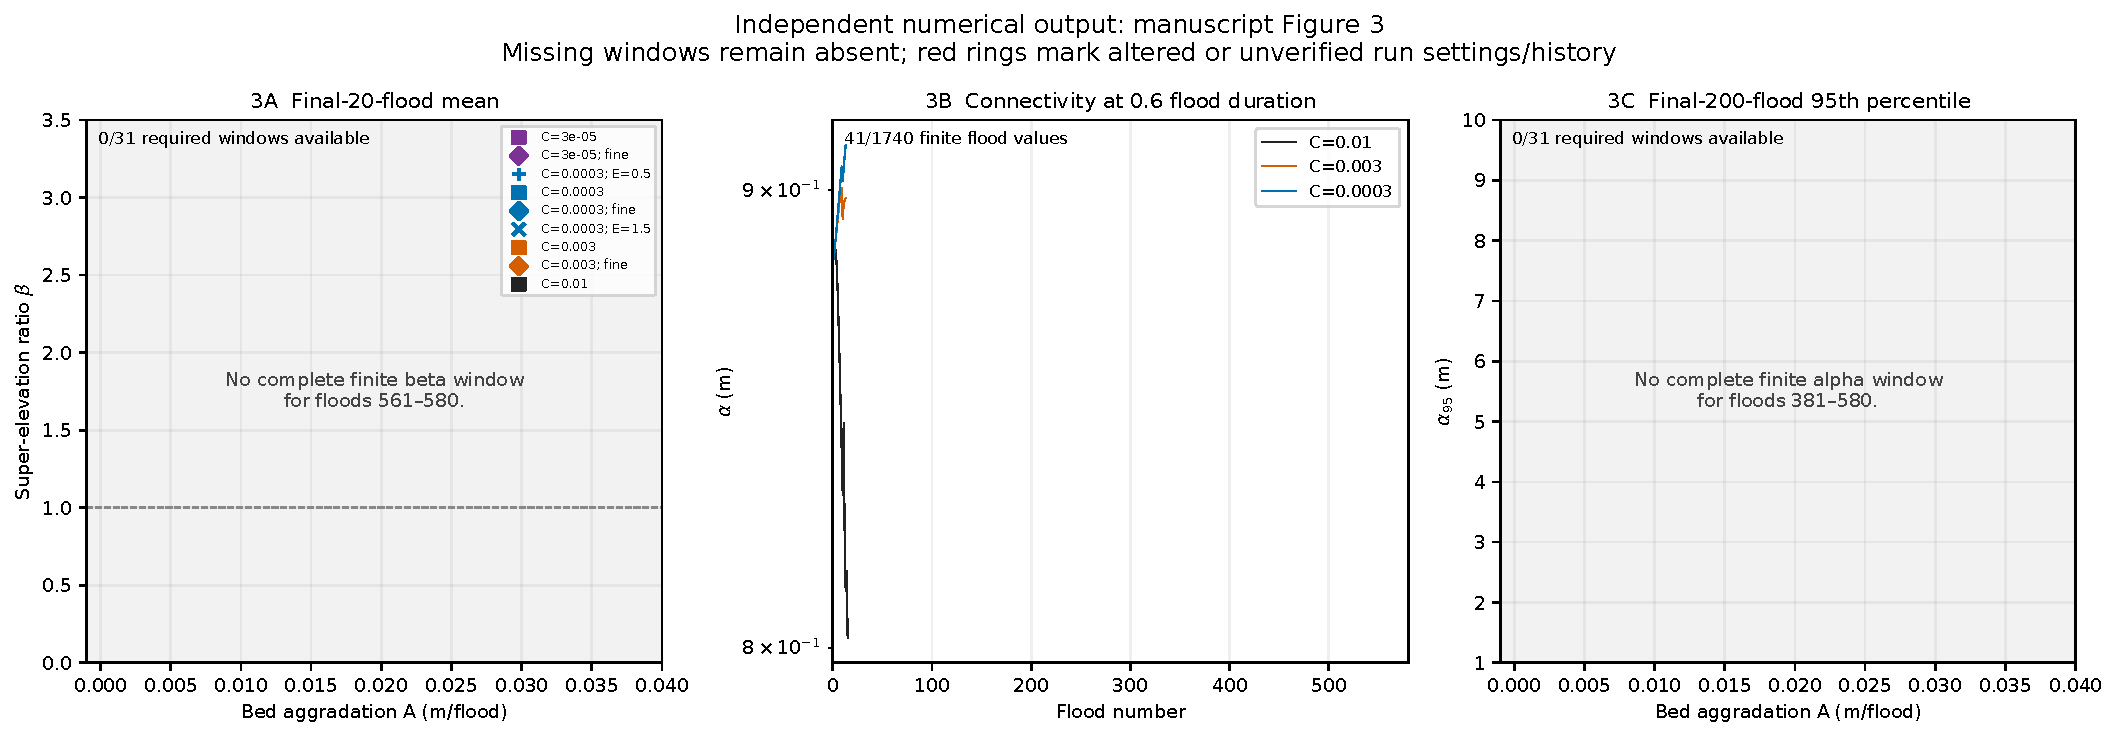
\includegraphics[width=\linewidth,height=4.4in,keepaspectratio]{figures/figure3.pdf}
\end{center}
\textbf{Figure 2.} Existing frozen manuscript-Figure-3 preview. Panel B contains 41 of 1,740 requested $\alpha$ values from runs 7, 15, and 20; A and C have no complete requested windows. $\alpha$ has units of metres; $\beta$ is dimensionless; horizontal time is flood number. Missing histories are left blank. Source: \file{figures/figure3.pdf}, bound to \file{validation/production-preview-20261011/}. A plotted frame is not successful reproduction.

\textbf{Published findings.} Mature ridge sections, changing overbank-deposit patterns, the dependence of $\beta$ on aggradation and sediment load, erodibility effects, and late-stage confinement remain untested. No central mature-ridge finding is quantitatively recovered or securely contradicted. Generic overbank deposition is recovered qualitatively; its similarity does not establish the published mechanism or spatial pattern.

For common floods 1--13, the independently recomputed population standard deviations of $\alpha$ are 0.00815, 0.00476, and 0.02452 m for increasing sediment-loading coefficients in runs 7, 15, and 20. Maxima are 0.91055, 0.90055, and 0.88649 m. Thus early peaks decrease with loading and variability is not monotonic. This does not recover the anticipated mature-ridge trend; the short initial interval cannot falsify it. Near-unit inundated-bank fractions also prevent interpreting $\alpha$ alone as evidence for localized breaches.

Requested sections begin at flood 50, deposit maps at flood 61, and final statistical windows at floods 381 or 561. The 31 current summaries contain 19--27 completed floods (timestamped inventory in the Appendix); no newer live output was substituted into these frozen figures.

\newpage
\textbf{Ranked unresolved obstacles.}

1. \emph{Numerical limitations.} Strong grid dependence changes storage, deposition, and the raster representation of banks. Conservative geometry transfer does not preserve uniform water depth or establish accurate migration. Longer integrations can amplify these differences.

2. \emph{Incomplete specification and model departures.} Sediment concentration units, exchange with the bed, entrainment, and migration closures could change ridge growth. Resolving acceptable assumptions requires human scientific judgment or missing information, not further autonomous implementation by default.

3. \emph{Duration and missing analysis.} Required late windows and spatial profiles are absent. Longer computation addresses duration only. A previous remapping implementation overdrew donor sediment and was replaced; corrected consistency checks address that error, not all remaining accuracy questions. Repeating unconstrained runs before resolving these issues has low expected return.

\textbf{Proposed spending decision.} One existing-data review is the smallest useful next step. This is a proposal, not authorization.

\begin{center}\small
\begin{tabularx}{\linewidth}{>{\raggedright\arraybackslash}p{1.25in}X}\toprule
Scientific question & Can this approximation support one defensible observable despite grid sensitivity and uncertain closures?\\\midrule
Specific work & A fluvial scientist and one agent review saved resolution/closure results and reconcile consequential assumptions with written methods. No new model runs or code changes.\\
Deliverable & A short decision memo selecting one observable and an explicit accuracy requirement, or recommending termination.\\
Success criterion & Every selected observable has a stated physical interpretation, numerical-error requirement, and bounded test that could accept or reject its use. Unresolved specifications are identified explicitly.\\
Principal risk & Existing evidence cannot separate discretization, bank geometry, and physical-closure effects. Human judgment or author clarification remains necessary.\\
Agent ceiling & 20,000 additional tokens, one review cycle. A discretionary cap, not an empirically calibrated estimate; no verified billing or applicable pricing supports a dollar estimate.\\
Compute ceiling & One CPU-hour for existing-file analysis; zero simulation hours. This is an operational cap, not a solver-runtime forecast.\\
Stopping condition & Stop at either ceiling, or when missing physical information prevents a defensible observable. Any simulation or implementation work requires a separate decision.\\\bottomrule
\end{tabularx}
\end{center}

Agent activity lacks audited task-level spending attribution. Historical runtime observations on a shared CPU host do not establish a reliable 580-flood completion estimate. Neither sunk cost nor elapsed computation justifies continuation.

No agents, model development, parameter searches, or simulations were launched for this assessment. Existing background calculations were not stopped. Remaining checks include independent full-budget reconstruction, coupled spatial and temporal convergence, mature-ridge comparisons, and a complete provenance audit. No prohibited author code, outputs, digitized inputs, or copied result figures were found in the inspected evidence; that limited inspection is not an exhaustive provenance guarantee.

\clearpage
{\large\bfseries Appendix: panel inventory and evidence trail}\par
\small
All 13 main-manuscript panels are listed individually below. N = requested independent numerical data absent; P = partial independent data. \emph{Quantitative agreement is unestablished for every panel.} No schematic is counted as a numerical result. The locally retained supplement text has DR1 methods and DR2 a parameter/results table, with no supplementary figure panels; its figure reference points to manuscript 1E. No supplementary numerical panel is therefore omitted from the original scope.

\texttt{P/} below means \file{validation/production-preview-20261011/data/}. Each cited run contains \file{parameters.txt} and \file{summary.csv}; these establish configurations and early histories, not missing requested snapshots. Plot paths are relative to the project root. Figure 1 and 2 placeholders were inventoried, not visually reassessed here.

\begin{tabularx}{\linewidth}{l>{\raggedright\arraybackslash}p{2.0in}lX}\toprule
Panel & Quantity and required floods & Status & Data; plot; principal limitation\\\midrule
1A & Event deposit thickness; 61 & N & \texttt{P/run11/}; \texttt{figures/figure1.pdf}; snapshot absent\\
1B & Event deposit thickness; 251 & N & \texttt{P/run11/}; same plot; snapshot absent\\
1C & Event deposit thickness; 501 & N & \texttt{P/run11/}; same plot; snapshot absent\\
1D & Event deposit thickness; 562 & N & \texttt{P/run11/}; same plot; snapshot absent\\
1E & Deposit thickness/interface; 562 & N & \texttt{P/run17/}; same plot; snapshot absent\\
1F & Event deposit thickness; 562 & N & \texttt{P/run03/}; same plot; snapshot absent\\
2A & Section elevation; 50,225,400,580 & N & \texttt{P/run22/}; \texttt{figures/figure2.pdf}; all four snapshots absent\\
2B & Section elevation; 50,225,400,580 & N & \texttt{P/run10/}; same plot; all four snapshots absent\\
2C & Section elevation; 50,225,400,580 & N & \texttt{P/run03/}; same plot; all four snapshots absent\\
2D & Section elevation; 50,225,400,580 & N & \texttt{P/run15/}; same plot; all four snapshots absent\\
3A & Mean $\beta$ versus aggradation; 561--580 & N & \texttt{P/run01/}--\texttt{run31/}; \texttt{figures/figure3.pdf}; 0/31 complete windows\\
3B & $\alpha$ each flood, day 12; 1--580 & P & \texttt{P/run07/}, \texttt{run15/}, \texttt{run20/}; same plot; 41/1740 values, early statistics in main text\\
3C & 95th-percentile $\alpha$; 381--580 & N & \texttt{P/run01/}--\texttt{run31/}; same plot; 0/31 complete windows\\\bottomrule
\end{tabularx}

\textbf{Comparison targets, not achieved agreement.} The existing comparison procedure retains written erodibility effects of approximately $+15\%$ and $-6.5\%$, a fine-load case exceeding $\beta=1$, and tendencies with aggradation and loading. None has a valid late-window comparison. Manuscript section-relief ranges in the comparison documentation are approximate visual readings, not digitized inputs, uncertainty intervals, or calibrated acceptance bands. They were not remeasured for this report. There are no claimed errors against those ranges.

\textbf{Definitions and commands.} \file{docs/panels.csv} records all configurations and data/plot commands; \file{figures/panel_status.csv} records plot inputs. \file{docs/comparison.md} defines comparisons and sampling windows. \file{figures/comparison.json} retains pending comparisons. Independent generation and agreement are separate: status P for 3B indicates available early data, not successful scientific reproduction.

\clearpage
{\large\bfseries Appendix: supporting files and inspection limits}\par
\small
\textbf{Evidence references (relative to repository root).}\par
\begin{tabularx}{\linewidth}{>{\raggedright\arraybackslash}p{1.35in}X}\toprule
Purpose & Files and inspection scope\\\midrule
Model specification & \file{docs/specification.md}, \file{docs/implementation.md}, \file{docs/scientific-audit.md}, \file{config/physics.txt}. Methods documentation inspected; selected settling/deposition source read in \file{src/sediment.hpp}; no full source audit.\\
Numerical checks & \file{docs/numerical-validation.md}, \file{validation/remap-full-check.txt}, \file{docs/first-flood-validation.md}. Saved results inspected; tests not rerun.\\
First-flood data & \file{validation/first-flood-audit-002/resolution-inputs.tar.xz}, \file{two-resolution.json}, \file{capture-provenance.json} in the same directory. Twenty-four archived members and figure inputs verified.\\
Additional sensitivities & \file{validation/first-flood-audit-002/fine-grid.json}, \file{time-step.json}, \file{threshold.json}, \file{concentration.json} in that directory, with capture records and input archives. No full numerical replay in this assessment.\\
Figure bindings & \file{figures/first_flood_validation_manifest.json}; \file{figures/plot_manifest.json}; frozen preview \file{validation/production-preview-20261011/}. Two included figures visually inspected.\\
Early statistics & \file{docs/early-production-assessment.md}; frozen run07, run15, run20 summaries. Common-13-flood maxima and population standard deviations independently recomputed.\\
Runtime and activity & \file{docs/runtime-observation.md}; process logs and provenance records in validation archives. Historical observations only; no audited dollar accounting or complete agent-record review.\\
Assessment audit & \file{validation/assessment-evidence-20261012/inventory.json}, \file{checks.json}, and \file{README.md}. File hashes, current coverage snapshot, preserved untracked evidence, and check scope.\\\bottomrule
\end{tabularx}

\textbf{Preservation and provenance.} The initially untracked directories were:\par\file{validation/runs/}\par\file{validation/.threshold-render-check-sg7jvor8/}\par The former contains older, mixed-completion validation outputs; it is not the corrected archive used for Table 1. Its 30 files, including scientific checkpoints, are preserved in \file{validation/assessment-evidence-20261012/legacy-validation-runs.tar.xz}. The latter contains report-rendering checks, including deliberately corrupted-input fixtures. Its 20 unique files are preserved in \file{unique-renderer-checks.tar.xz} in the same evidence directory; 26 byte-identical copies of project files are omitted from that archive. These fixtures are validation evidence, not model results. Originals remain untouched.

\textbf{Coverage and publication.} The timestamped inventory records completed-row counts and hashes of 31 evolving production summaries under \file{tmp/full-rebuild-002/workspace/data/}. This is a coverage observation, not an audit of their physical validity. Frozen figures retain their original shorter histories. The upload includes tracked source, configurations, plots, frozen data archives, earlier reports, this assessment, and preserved historical evidence. Evolving temporary workspaces, executables, build products, downloaded publication sources, and credentials are excluded. Scientific checkpoints inside provenance archives are data, not executables.

\textbf{Reference.} Nicholas, A. P., Aalto, R. E., Sambrook Smith, G. H., and Schwendel, A. C. (2018), Hydrodynamic controls on alluvial ridge construction and avulsion likelihood in meandering river floodplains, \emph{Geology}, 46, 639--642; GSA Data Repository 2018219, DR1 and DR2. Written descriptions and published figures are specifications/comparison references only; no author output is used as an independently generated result.

\textbf{Build.} From the repository root, run \texttt{bash} \file{report/build_progress_assessment.sh}; it compiles twice with caches confined to the project. The delivered build was compiled in the ignored project-local \file{tmp/progress-assessment-build/}; only source and final PDF are deliverables. Main report: pages 1--4; appendix: pages 5--6.
\end{document}
